\documentclass[12]{article}
\title{%
	Design and Development of \\
	Hydraulically Actutated Autonomous Nurse (HYAAN)
	\large \\e-Yantra Ideas Competition\\
	}

\author{Kaushik Balasundar*, Aby J Kottoor, Akash S Nambiar, Shwetha D}
\usepackage{graphicx}
\usepackage[margin=0.5in]{geometry}
\graphicspath{{C:\Users\kaush\Desktop\Hyaan\e-YIC\Latex_report\flowchart.jpg}}
\begin{document}
	
	\pagenumbering{gobble}
	\maketitle
	\newpage
	\pagenumbering{roman}
	\setlength{\parindent}{1cm} % Default is 15pt.
	
	\section{Introduction/Motivation}
% \section{Introduction/Motivation}
	The general shortage of nursing staff worldwide is an aspect which is beginning to have a detrimental impact on hospitals, nursing professionals and the patients. Musculoskeletal injuries are predominant among nursing staff due to labour intensive physical tasks like lifting and repositioning patients multiple times on a daily basis. In some hospitals where there is a severe shortage of nursing staff, a nurse may need to do this process of turning patients up to 60 times a day, which exert a great deal of physical stress on the nursing staff. Furthermore, lifting a patient cannot be done by a single nurse and requires at least two nurses. Consequently, another set of patients are left unattended. It is estimated that India is at a shortage of 2.5 million nurses ~\cite{etimes} and by 2030, India will need an estimated 6 million nurses.  Therefore, there is a need to develop a lifting and turning mechanism which increases nurses’ efficiency, reduces their occupancy-related injuries, reduces patient rehabilitation time, ubiquitous for the entire ward, offers autonomous mobility and intelligence while being cost efficient. 
	
	\section{Market Research/Literature Survey}
	Previous works encompass multiple approaches including the use of human-type arms for transferring a patient, use of board type arms with endless conveyer belts, simple and small bed fixed on the robot arms and wheelchair-to-bed convertibles ~\cite{Bostelman}. The RIBA robot ~\cite{Mukai} is a humanoid robot with human type arms designed to perform heavy physical tasks requiring human contact, under constant human supervision, but payload limited to 60 kg. On similar lines, the RoNA system ~\cite{Ding} has a human-like upper body which includes two dexterous arms, torso, and head. Each arm has 7 actuated joints including 3 shoulder rotary joints, 2 elbow joints, 1 flipper and 1 forearm conveyor joint. The Bear robot is designed to lift 500lbs and move at approximately 10 miles per hour developed for extraction of patients from battlefield. Traditionally, there have been several other approaches used include patient pivot, Hoyer lift ~\cite{Hindawi} and C-Pam~\cite{Wang}. 
	
	
	\section{Requirements}
		\subsection{Hardware Requirements}
		1.	Hydraulic actuation system (3x double acting cylinders, appropriate vales and pump)\\
		2.	Kinect Camera \\
		3.	Wide angle lens camera\\ 
		4.	Hub motor with wheels\\
		5.	Power source (Lipo battery for motors and DC rectification unit for AC-DC conversion)\\
		
		\subsection{Software Requirements}
		1.	Robot Operating System \\
		2.	Snowboy.kitt.ai platform for hot word detection \\
		3.	Google Inception V3 pretrained model for posture classification \\
		4.	OpenCV 
		
	\section{Implementation}
	
		The overview for the methodology adopted to achieve an optimally functional solution to the described problem statement is as follows: \\
		
	\begin{itemize}
	
		\item Evaluation of the requirements of the robot on consultation with the end users (hospital doctors, nurses and patients). Upon appropriate evaluation of the market needs, the most important requirements will be narrowed down.
		
		\item Each requirement will be mapped to an engineering problem to be solved. The proposed objectives will be initially be achieved by developing a CAD model using Fusion360 and evaluating the kinematic and dynamic feasibility. This step will involve multiple iterations and continuous modifications to arrive at the most efficient mechanism to carry out the desired functions. 
		
		\item Since safety is of primary importance, we will opt for hydraulic actuation due to its ability to retain hydraulic pressure and thus not drop the patient in the case of power failure. 
		
		\item The hydraulic circuit, pump and hub motor specifications needs to be calculated for the actuation and locomotion systems respectively. We will then develop the necessary software tools to be implemented in the robot such as computer vision aided pose estimation of the patient, UI design, sensor interfacing with microcontroller, and autonomous navigation using 3D cameras.  
		
		\item The computer vision model to detect patient pose will be deployed using customized dataset on the pretrained Google inception V3 model. The humanoid head which houses the camera used for pose-detection will be designed using Fusion 360. 
		
		\item The next stage will include the manufacturing of the customized hydraulic system, procurement of raw materials, bearing and fasteners for the frame, and fabrication of the 1:1 scale model according to the optimized CAD model. 
		
		\item Certain components which require customized design fabrication will be 3D printed (e.g., the humanoid head camera housing). 
		
		\item In the final stage, the developed software and hardware will be integrated to function in harmony. The entire system will then be rigorously tested to identify mechanical, software and control flaws which will be eliminated through multiple optimization iterations.  
		
	
	\end{itemize}

\section{Flowchart}

	\begin{figure}[hbt!]
		\centering
		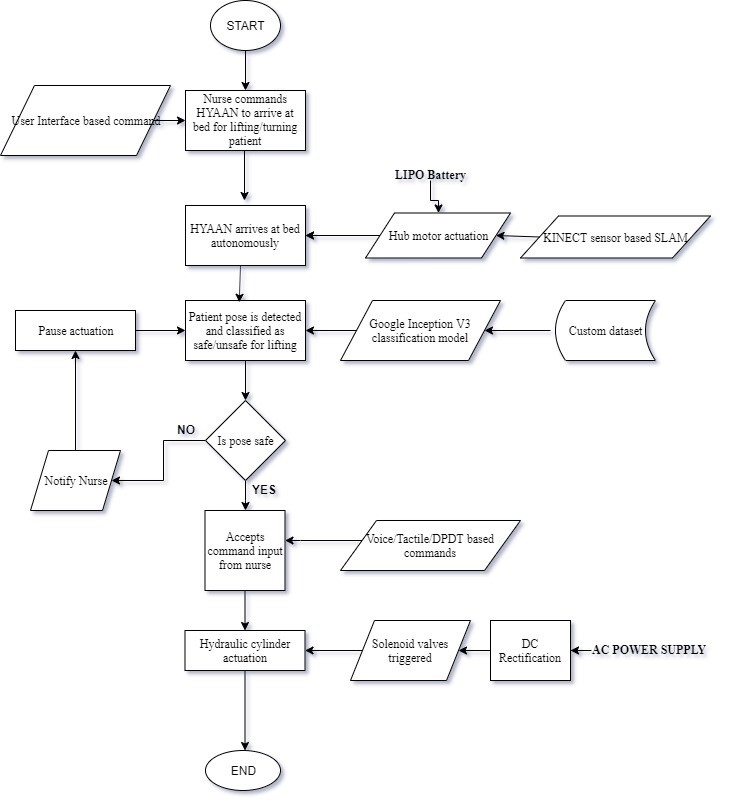
\includegraphics[scale=0.5]{Flowchart.jpg}
		\caption{Funcational Flowchart}
		\label{image_1}
	\end{figure}
		
		
\section{Feasibility}
One of the major constraints in the current solutions available is that they are extremely expensive. There is a need to develop humanoid robots which can be mass-produced and thereby become affordable for a plethora of applications. As a result, we are using commercially available off-the-shelf sensors are used in the robot. Our solution has no drive mechanisms and therefore, there are no issues of patient safety being compromised due to impact forces caused from backlash and inertia. Hydraulic systems also have the additional advantage of being able to retain the hydraulic pressure even in the case of a power failure and hence the patient will not be dropped in such scenarios. To make control of the robot more intuitive, we will employ tactile guidance and teleoperation-based control. These design decisions will make our model more feasible for practical use as compare to existing solutions available in the market. 
\begin{thebibliography}{9}
	\bibitem{etimes} https://economictimes.indiatimes.com/industry/healthcare/biotech/healthcare/india-facing-shortage-of-600000-doctors-2-million-nurses-study/articleshow/68875822.cms?from=mdr
	\bibitem{Bostelman}
	Roger Bostelman and James Albus, “Robotic patient lift and transfer”, National Institute of Standards and Technology USA
	\bibitem{Mukai}
	Toshiharu Mukai, Shinya Hirano, Hiromichi Nakashima, Yo Kato, Yuki Sakaida, Shijie Guo and Shigeyuki Hosoe, “Development of a nursing-care assistant robot RIBA that can lift a human in its arms,” in the 2010 IEEE/RSJ International Conference on Intelligent Robots and Systems October 18-22, 2010, Taipei, Taiwan.
	\bibitem{Ding}
	Jienan Ding, Yi-Je Lim, Mario Solano, Kevin Shadle, Chris Park, Chris Lin, John Hu, “Giving patients a lift – the robotic nursing assistant (RONA),” 978-1-4799-4605-1/14/2014 IEEE.
	\bibitem{Hindawi}
	Design and user evaluation of a wheelchair mounted robotic assisted transfer device: Hindawi Publishing Corporation Biomed Research International Volume 2015, Article ID 198476, 9 pages http://dx.doi.org/10.1155/2015/198476
	\bibitem{Wang}
	Hongbo Wang and Fumio Kasagam, “A patient transfer apparatus between bed and stretcher,” IEEE Transactions on Systems, Man, and Cybernetics—Part B: Cybernetics, Vol. 38, No. 1, February 2008.
\end{thebibliography}
\end{document}